\documentclass[11pt]{article}
\usepackage[utf8]{inputenc}
\usepackage[T1]{fontenc}
\usepackage{lmodern}
\usepackage{amsmath, amssymb}
\usepackage{booktabs}
\usepackage{hyperref}
\usepackage{geometry}
\usepackage{graphicx}
\usepackage{xcolor}
\usepackage{listings}
\geometry{margin=1in}

\begin{document}

\title{Anti-PD-1 Monoclonal Antibody Optimization: A Computer-Aided Drug Discovery Using the Rosetta Suite}
\maketitle

\section{Abstract}

Computer-Aided Drug Discovery (CADD) accelerates the identification and optimization of drug candidates by predicting interactions between therapeutic molecules and their biological targets. This study demonstrates the application of Structure-Based Drug Discovery (SBDD) techniques, specifically using the Rosetta suite, to design and optimize therapeutic antibodies targeting the PD-1 receptor—a key regulator of immune responses whose inhibition can enhance anti-cancer activity. Pembrolizumab, an FDA-approved PD-1 inhibitor, was selected as the lead candidate, and detailed interaction analysis revealed its overall favorable binding energy and stable interaction profile with the receptor. However, specific residues in Pembrolizumab—namely, the 53rd residue on the light chain (TYR) and the 59th residue on the heavy chain (ASN)—were identified as engaging in unfavorable interactions that destabilized the complex. To address these issues, we employed two complementary mutation strategies: a targeted point mutation to directly substitute the problematic residues, and a broader CDR mutation approach aimed at optimizing the overall interface. The mutagenesis significantly improved the stability and binding affinity of the Pembrolizumab-PD-1 complex. This study highlights the potential of Rosetta-based CADD methods to refine therapeutic antibodies and accelerate the development of more effective cancer therapies.

\section{Introduction}

Drug discovery has traditionally been a lengthy, resource-intensive process requiring years of research, development, and testing before a promising compound can reach clinical trials \cite{DiMasi2003,Paul2010}. In recent years, Computer-Aided Drug Discovery (CADD) has emerged as a transformative alternative by harnessing advanced computational techniques to predict interactions between small molecules (or proteins) and their biological targets \cite{Kitchen2004,Lionta2014}.  This virtual screening approach dramatically accelerates the early-stage identification and later-stage optimization of promising candidates, while significantly reducing the time and costs associated with traditional methods \cite{Sliwoski2014}.

CADD combines two complementary approaches: Structure-Based Drug Discovery (SBDD) and Ligand-Based Drug Discovery (LBDD) \cite{Kuhn2016}. SBDD uses three-dimensional structural information of target biomolecules to guide drug design, employing techniques like molecular docking and dynamics simulations to evaluate compound binding and predict affinities \cite{Kitchen2004}. This approach enables rational molecule design with enhanced interaction profiles. In contrast, LBDD relies on known ligand features and activities, using methods such as quantitative structure-activity relationship (QSAR) modeling to predict bioactivity even without detailed target structures \cite{Kuhn2016}. Integrating these approaches creates a synergistic strategy for drug discovery, with SBDD providing molecular interaction insights and LBDD refining candidate selection by predicting pharmacological properties like efficacy and toxicity \cite{Moult2019}. This combination accelerates drug development by reducing early-stage failures and streamlining candidate optimization \cite{DiMasi2003,Paul2010}. In this study, I will focus on applying SBDD with the Rosetta suite to design and optimize therapeutic antibodies targeting the Programmed Cell Death Protein 1 (PD-1) receptor.

Among the many computational tools available for CADD, Rosetta stands out as a particularly powerful and widely used software suite for SBDD, especially in the fields of protein design and antibody engineering \cite{Leaver-Fay2011}. Rosetta is a computational framework for biomolecular modeling, structure prediction, and drug discovery, offering a comprehensive suite of tools that integrate flexible docking, de novo protein design, and ligand binding optimization \cite{leman2020}. Unlike traditional molecular docking software, Rosetta employs Monte Carlo-based sampling and energy minimization to improve the accuracy of protein-ligand interactions \cite{Alford2017, meiler2006}. One of its key advantages is the ability to model induced-fit binding and backbone flexibility, making it especially useful for targets like PD-1, where conformational changes influence ligand binding \cite{park2019}. Due to its versatility and modularity, Rosetta is a valuable tool for SBDD, allowing researchers to screen, refine, and optimize new PD-1 inhibitors within a single platform \cite{leaver2013, baek2021}.

PD-1, the focus of this study, is a transmembrane receptor expressed on activated immune cells, including T cells and B cells, and plays a crucial role in maintaining immune homeostasis by regulating T-cell activation. Under normal physiological conditions, PD-1 functions as an essential checkpoint, preventing autoimmunity by limiting excessive immune responses \cite{Dong2002}. However, many tumor cells exploit this pathway by overexpressing PD-L1, the ligand for PD-1, which binds to PD-1 and inhibits T-cell effector functions, allowing tumors to evade immune surveillance \cite{Topalian2015}. Structurally, PD-1 is a 288–amino acid protein organized into three main regions: an extracellular immunoglobulin variable (IgV) domain (approximately residues 22–170), a single transmembrane segment, and a cytoplasmic tail containing key signaling motifs \cite{Tan2016,Chen2019}. The IgV domain plays a key role in maintaining the protein's structural integrity and serves as the primary binding interface for ligands such as PD-L1, PD-L2, and potential PD-1 inhibitor drugs.

Given the critical role of PD-1 in immune regulation and cancer immune evasion, it serves as an ideal target for therapeutic antibody design. In this study, I will explore the use of Rosetta to design and optimize novel antibody candidates targeting PD-1. By leveraging the various modules available in Rosetta, I aim to refine the interaction between the antibody and PD-1, enhancing its binding affinity and specificity to improve therapeutic efficacy. The goal is to demonstrate how CADD techniques, particularly those enabled by Rosetta, can accelerate the development of PD–1–based therapies and improve their potency and durability, overcoming current limitations in the treatment of cancer.

\section{Methods}

\subsection{System and Software}

All computational analyses were performed on a machine running Ubuntu 10.04. The Rosetta 3.14 suite was used for computational antibody design and docking simulations \cite{Leaver-Fay2011}. Rosetta documentation is available at \url{https://docs.rosettacommons.org/docs/latest/getting_started/Getting-Started}. For descriptions of the commands, please refer to Supplementary. Chimera 1.18 was employed for structural visualization, analysis, and structure editing \cite{pettersen2004}. Python scripts used to analyze the data and output PDB files are available at \url{https://github.com/gilmore307/Molecular-Docking}.

\subsection{Structure Preparation}  
To obtain a complete PD-1 model for computational analysis, structural data from multiple sources were integrated. The PD-1 receptor was reconstructed by combining models from PDB ID: 5GGS \cite{lee2016} (which lacks residues 25-32) and PDB ID: 5WT9 \cite{tan2017} (which lacks residues 85-93 and 143-146) using Chimera 1.18 to complement the missing parts. The combined structure was then relaxed using the Rosetta Relax protocol.

The structures of three FDA-approved PD-1 inhibitors were extracted from their respective PDB entries: Pembrolizumab from PDB ID: 5GGS, Nivolumab from PDB ID: 5WT9 and Cemiplimab from PDB ID: 7WVM \cite{lu2022}. These structures were used for computational docking and comparative binding analyses in the subsequent steps.

\subsection{Docking Drug Molecules with the PD-1 Structure}  
To evaluate the binding affinity and interaction patterns of candidate drug molecules with the PD-1 receptor, molecular docking was performed using Rosetta's docking protocol. The docking protocol utilized a preprocessed and remodeled PD-1 structure, along with a ligand structure. The docking simulation was executed, and the binding affinity of the resulting complexes was analyzed to identify the most favorable binding pose based on the lowest energy conformation, representing the most stable PD-1-ligand interaction.

\subsection{Interaction Analysis and Energy Breakdown}  
The drug with the best docking interaction with PD-1, determined by the lowest binding energy, was selected as the template drug. The pose with the lowest binding energy was then used in subsequent steps for further interaction analysis.

Interaction Analysis was performed using Rosetta's InterfaceAnalyzer module, which evaluates the interface between the protein and the ligand. The module provides a detailed examination of the interaction energies, considering both van der Waals and electrostatic contributions at the protein-ligand interface. It helps identify critical contact residues and assess the overall stability of the ligand-protein complex. To gain more granular insights into the energetic contributions of individual amino acids, Rosetta’s ResidueEnergyBreakdown module was deployed. This tool breaks down the interaction energies on a per-residue basis, offering detailed information on which specific residues play pivotal roles in binding and their relative contributions to the binding affinity. This analysis is essential for identifying key residues that could be targeted for further optimization or mutagenesis studies.

\subsection{Point Mutation and CDR Mutation for Enhanced Binding Affinity}  

In the mutagenesis studies, specific mutations were introduced based on residues that exhibited unfavorable interactions, as identified in the previous energy breakdown step, where high interaction energies were observed. To address these issues and improve the binding profile of the drug, point mutations were performed using Chimera’s Rotamers tool with the Dunbrack 2010 library \cite{shapovalov2011}. For each mutated residue, the tool generated possible side-chain rotamers, and the rotamer with the highest probability was selected. 

The Complementarity-Determining Regions (CDRs) of the antibody were defined based on previous docking results, where regions closely interacting with PD-1 receptor were identified as the CDRs. To optimize these regions, the antibody\_designer module in Rosetta was used to perform sequence design on the defined CDRs. The design process involved mutating the amino acid sequences within the CDRs to enhance their binding affinity to PD-1, while maintaining the structural integrity of the antibody. Energy minimization and side-chain optimization were applied to ensure that the designed CDRs exhibited favorable interactions with the receptor. This process aimed to refine the antibody's ability to interact with PD-1 and improve its overall stability and binding strength.

After the mutations were introduced, the modified antibody molecule was re-docked with PD-1. The binding affinity and interaction profile of the mutated antibody were then compared with the original lead drug to assess any improvements in binding.

\subsection{Testing the Stability of the New Drug Molecule}  
To test the stability of the newly optimized drug molecule, the structure was scored using Rosetta's scoring function. This procedure provided an overview of the energy and stability of the antibody. The solvation energy and solvent-accessible surface area (SASA) of the antibody were also assessed to understand how the antibody interacts with its environment, especially in a biological system.

\section{Results}
\subsection{Molecule Docking of Lead Drugs} 

\begin{figure}[t]
\begin{center}
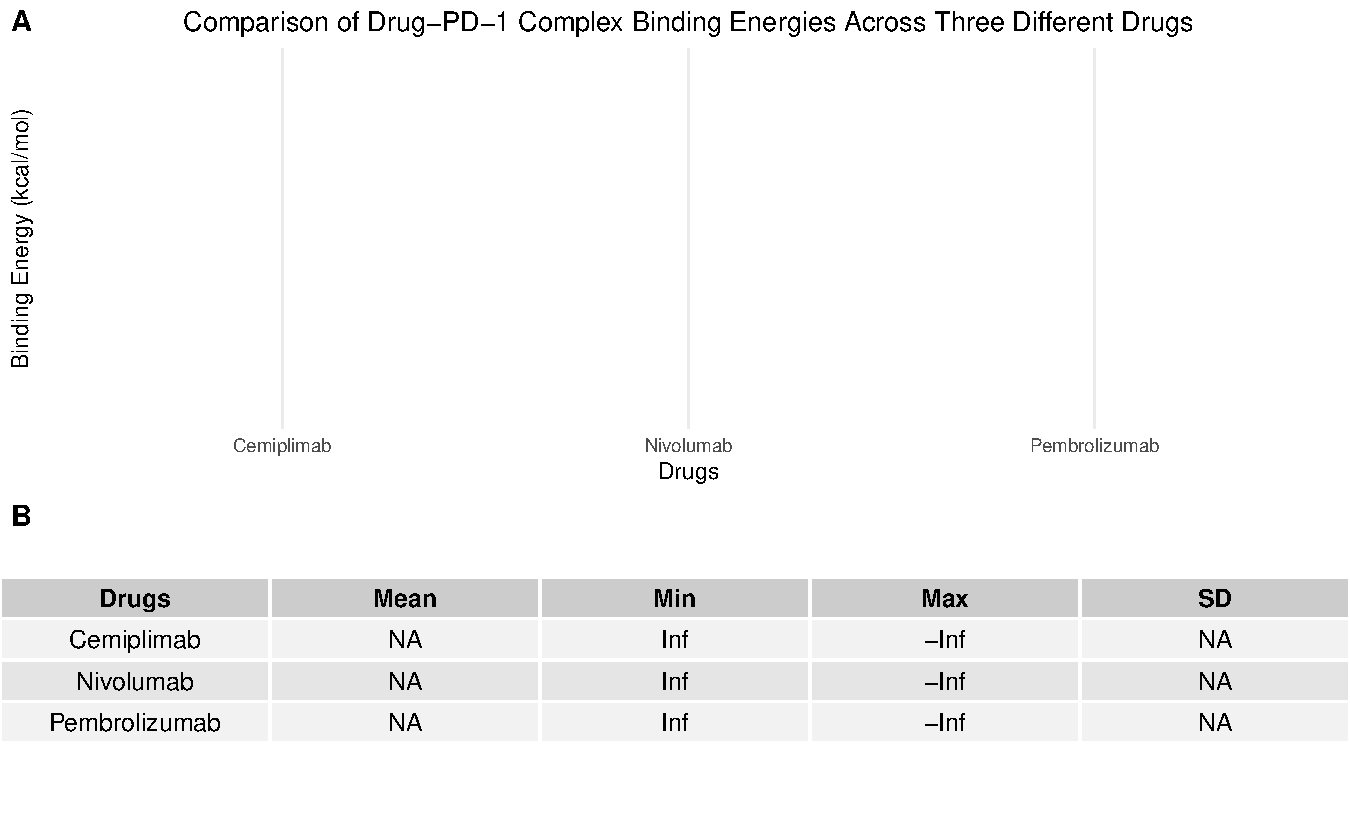
\includegraphics[width=0.8\textwidth]{Figure1.pdf}
\end{center}
\caption{Comparison of Binding Energies of Drug-PD-1 Complex Across Different Drugs}
\textbf{(a)} Box plot showing the distribution of binding energies (kcal/mol) for three PD-1 inhibitors: Pembrolizumab, Cemiplimab, and Nivolumab.
\textbf{(b)} Statistical summary of the binding energies, including mean, min, max, and standard deviation.
\label{fig:fig1}
\end{figure}

Molecular docking simulations were performed to investigate the binding interactions of several PD-1 inhibitors with the PD-1 receptor. Three lead drugs, including Cemiplimab, Nivolumab, and Pembrolizumab, were analyzed for their binding affinities to PD-1. The binding energies of each drug to PD-1 were computed, and their respective docking scores are summarized in Figure 1.

The binding energies of the drugs varied significantly, as depicted in Figure 1A, with the statistical summary of these values presented in Figure 1B. The most favorable binding energy was observed for Pembrolizumab ($-735.76$ kcal/mol in average), followed by Cemiplimab ($-388.64$ kcal/mol in average) and Nivolumab ($-233.40$ kcal/mol in average). Given that Pembrolizumab exhibited the lowest binding energy and the most stable interaction with PD-1, it was selected as the lead drug for further studies. The favorable binding profile of Pembrolizumab suggests strong inhibition potential, which may translate to enhanced therapeutic efficacy in PD-1 targeted therapies.

\subsection{Interaction Analysis of Pembrolizumab with PD-1}

\begin{figure}[t]
\begin{center}
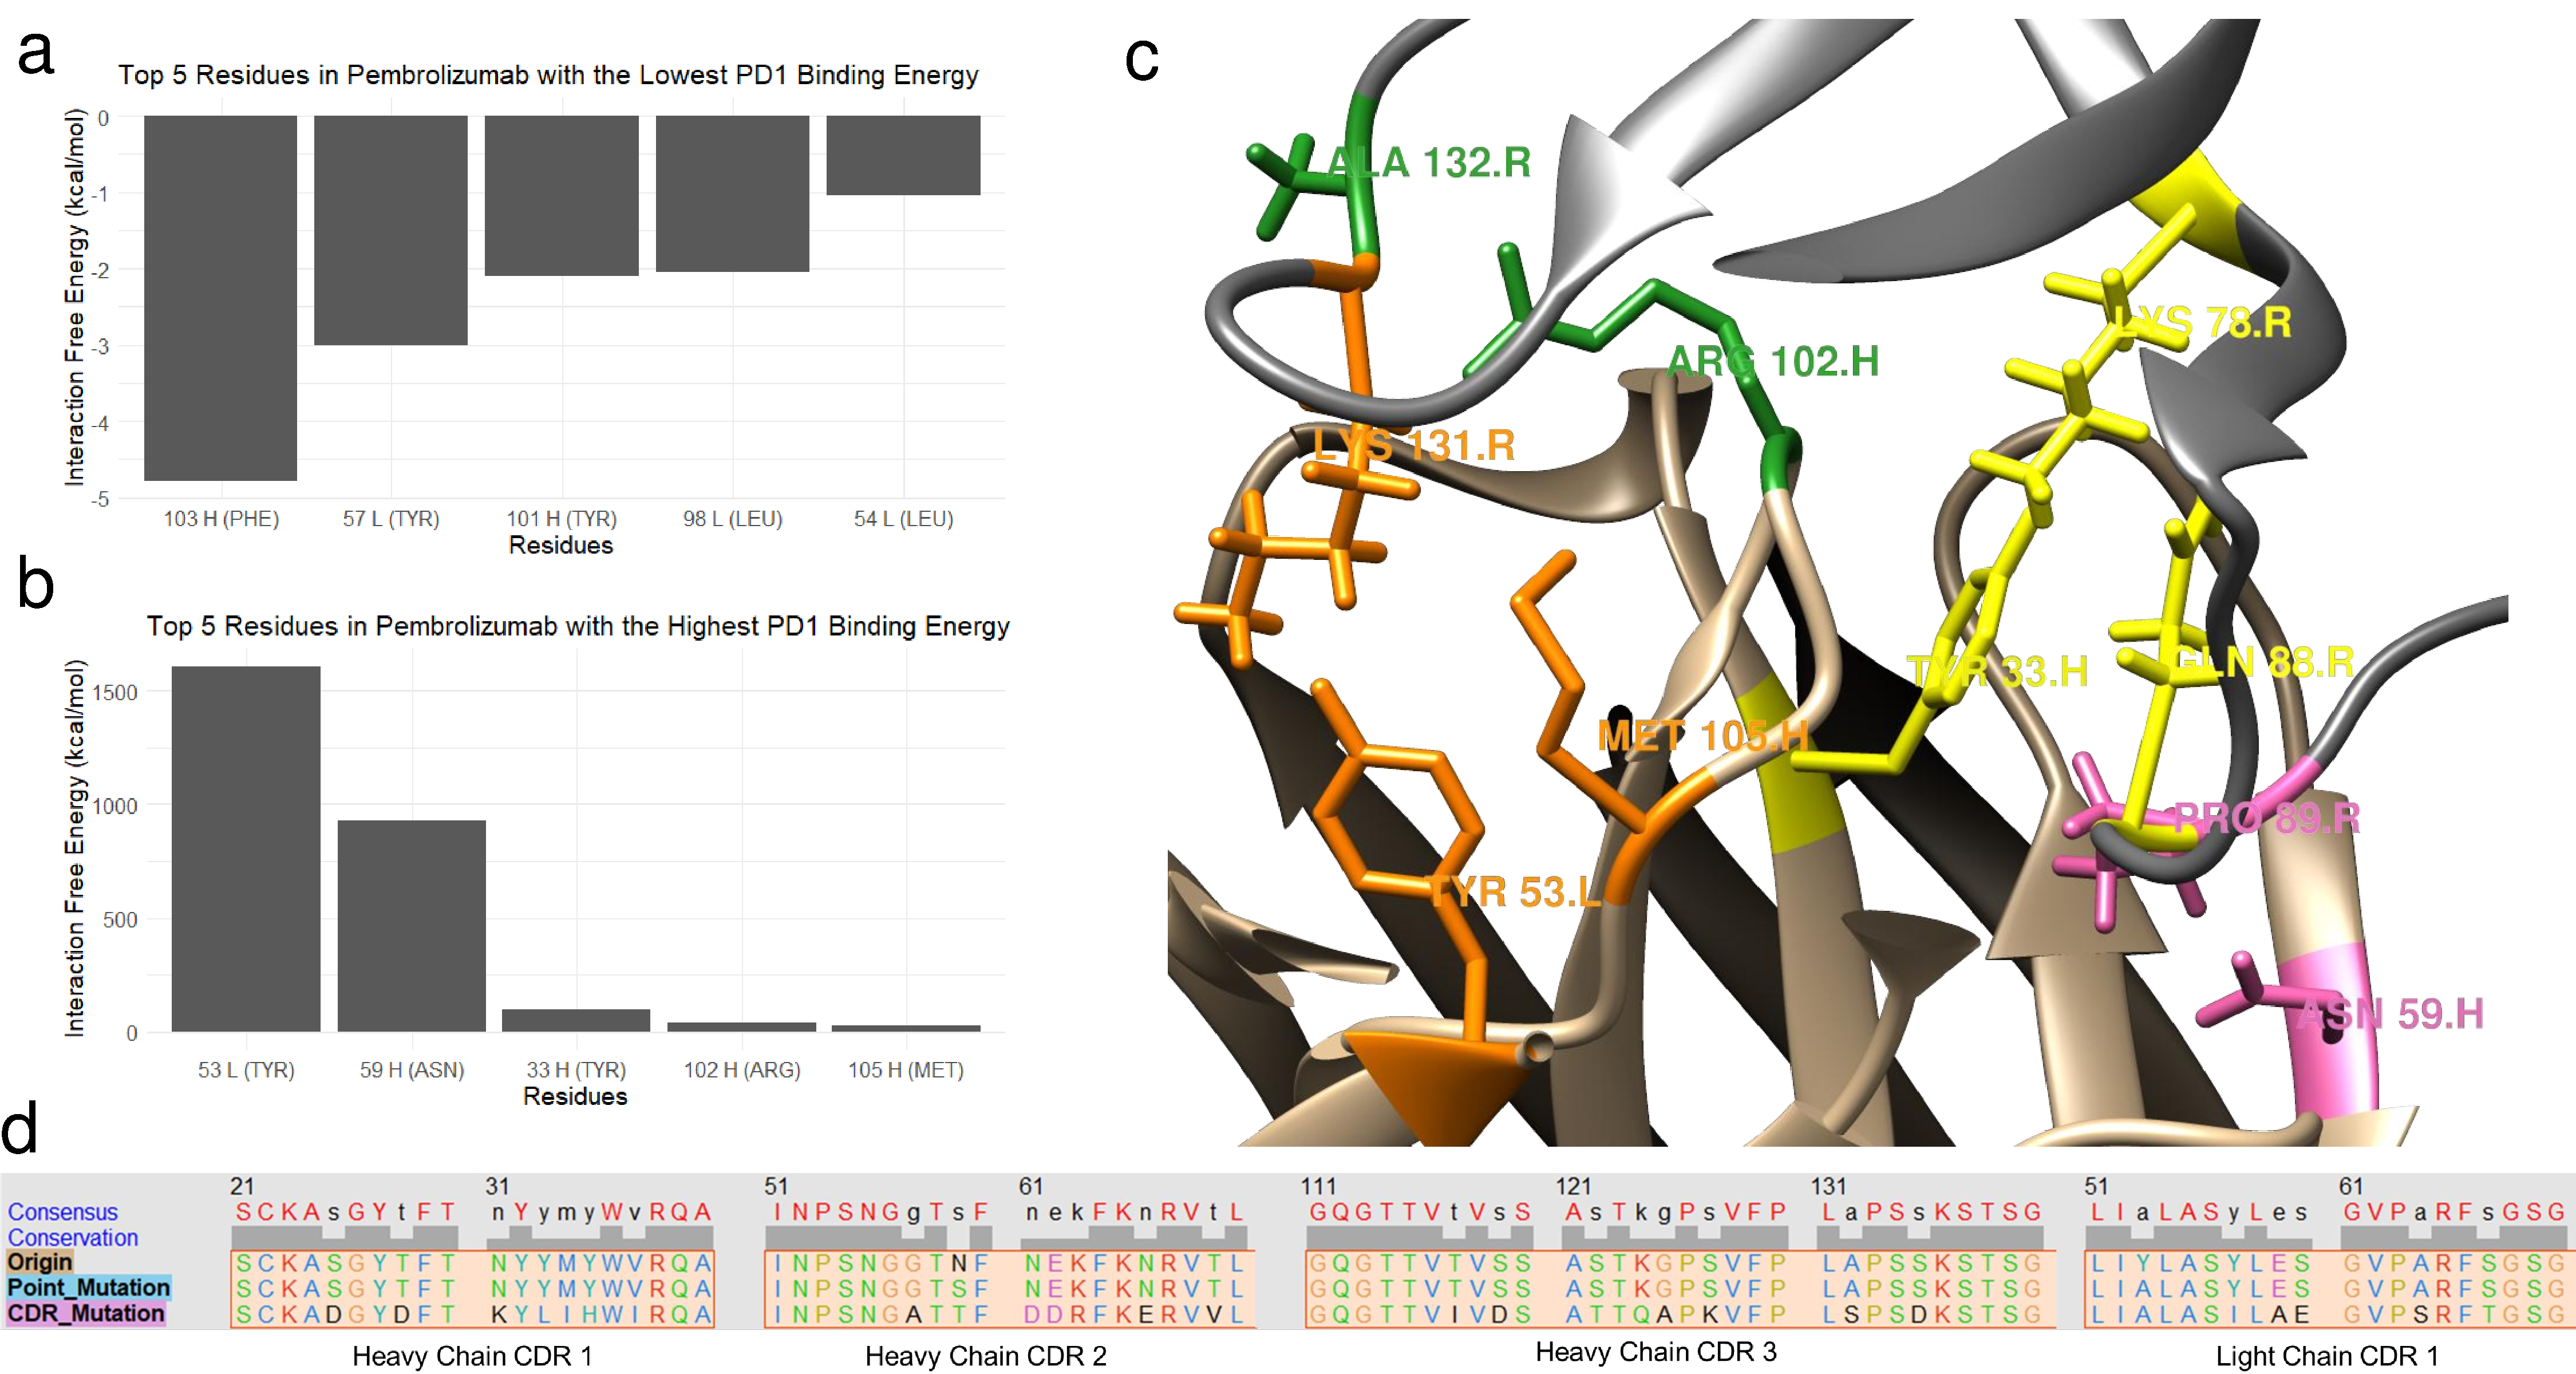
\includegraphics[width=0.8\textwidth]{Figure2.pdf}
\end{center}
\caption{Interaction Analysis of Pembrolizumab with PD-1.}
\textbf{(a)} The top 5 residues in Pembrolizumab with the lowest PD-1 binding energy, indicating the most favorable interactions. 
\textbf{(b)} The top 5 residues in Pembrolizumab with the highest PD-1 binding energy, suggesting destabilizing interactions. 
\textbf{(c)} Visualization of the binding interactions reveals four groups of high free energy interactions, highlighting destabilizing effects. Each group is in a different color. These include: 131 R (LYS) interacting with 53 L (TYR) (1604.238 kcal/mol) and with 105 H (MET) (29.518 kcal/mol), 59 H (ASN) interacting with 89 R (PRO) (927.142 kcal/mol), 33 H (TYR) interacting with 78 R (LYS) (79.722 kcal/mol) and with 88 R (GLN) (17.04 kcal/mol), and 102 H (ARG) interacting with 132 R (ALA) (34.979 kcal/mol).
\textbf{(d)} Residue alignment of CDRs between original Pembrolizumab, Pembrolizumab after point mutation and Pembrolizumab after CDR mutation.
\label{fig:fig2}
\end{figure}

The interaction between Pembrolizumab and PD-1 was assessed using the Rosetta ResidueEnergyBreakdown module. The analysis revealed key residues in Pembrolizumab that contribute to the stability and affinity of the complex. 

Specifically, as shown in Figure 2a, the top 5 residues with the lowest binding energies include 103 H (PHE) (the 103rd residue in the heavy chain of Pembrolizumab, which is Phenylalanine), 57 L (TYR), 101 H (TYR), 34 L (TYR), and 98 L (LEU). These residues form multiple favorable Van der Waals interactions with other hydrophobic residues in PD-1. For example, 103 H (PHE) interacts with residues like 64 R (VAL) and 81 R (ALA), with interaction energies of -1.973 kcal/mol and -1.272 kcal/mol, respectively. These interactions stabilize the complex by promoting favorable hydrophobic packing.

The interaction between Pembrolizumab and PD-1 revealed several residues that contribute to destabilizing interactions, primarily due to their significantly high binding energies. This is illustrated in Figure 2b, where 53 L (TYR), 59 H (ASN), 33 H (TYR), 102 H (ARG), and 105 H (MET) exhibit high binding energies that highlight unfavorable steric and electrostatic interactions. Specifically, as shown in Figure 2c, the interaction between 53 L (TYR) and 131 R (LYS) is destabilizing, with an energy contribution of 1604.238 kcal/mol, primarily driven by steric clashes and electrostatic repulsion. The polar aromatic TYR interacts unfavorably with the positively charged LYS, resulting in both steric clashes and increased electrostatic repulsion, making this interaction highly destabilizing. Similarly, the interaction between 59 H (ASN) and 89 R (PRO) contributes significantly to the destabilization of the complex, with a binding energy of 927.142 kcal/mol. This high energy arises from unfavorable electrostatic interactions and steric clashes between the polar ASN and the hydrophobic PRO, increasing repulsive forces and destabilizing the complex.

The high binding energies observed in these residues are mainly due to unfavorable steric clashes caused by their large side chains. To improve Pembrolizumab’s binding affinity and stability, we adopted a systematic, stepwise approach that first targeted unfavorable interactions through point mutations and then refined antigen binding via CDR sequence design. By first addressing the highly destabilizing residues through targeted point mutations, we minimized unfavorable steric clashes and electrostatic repulsions, creating a more favorable starting framework. With this structural refinement in place, we then focused on CDR sequence design to further optimize antigen binding, ensuring that changes introduced in the CDRs complement the improved backbone stability. This stepwise approach allowed us to systematically enhance Pembrolizumab’s binding affinity while maintaining an overall well-balanced and structurally stable antibody-receptor complex.

For point mutation, 53 L (TYR) will be substituted with 53 L (ALA) (Alanine) to reduce the steric clash and electrostatic repulsion with 131 R (LYS), while preserving the favorable hydrophobic interactions. For 59 H (ASN), we will substitute it with 59 H (SER) (Serine), a smaller, polar amino acid that will reduce the steric and electrostatic mismatch with 89 R (PRO), while maintaining the favorable interactions with 87 R (SER) and 88 R (GLN). By replacing these residues with smaller amino acids, we aim to reduce the high fa\_rep values (repulsive forces), which are a significant contributor to the high binding energies. 

To further refine Pembrolizumab and enhance its interaction with PD-1, we identified the Complementarity-Determining Regions (CDRs) in Pembrolizumab. Based on standard antibody structural conventions and previous residue energy breakdown analyses, heavy-chain CDRs were designated as H1 (residues 21-35), H2 (residues 51-70), and H3 (residues 111-140), while the light-chain CDR was identified as L1 (residues 51-70). The detail change on residue is shown in Figure 2d.

This mutation strategy will help minimize destabilizing interactions, improving the overall binding affinity and stability of the Pembrolizumab-PD-1 complex.

\subsection{Optimization Results of Pembrolizumab-PD-1 Interaction}

\begin{figure}[t]
\begin{center}
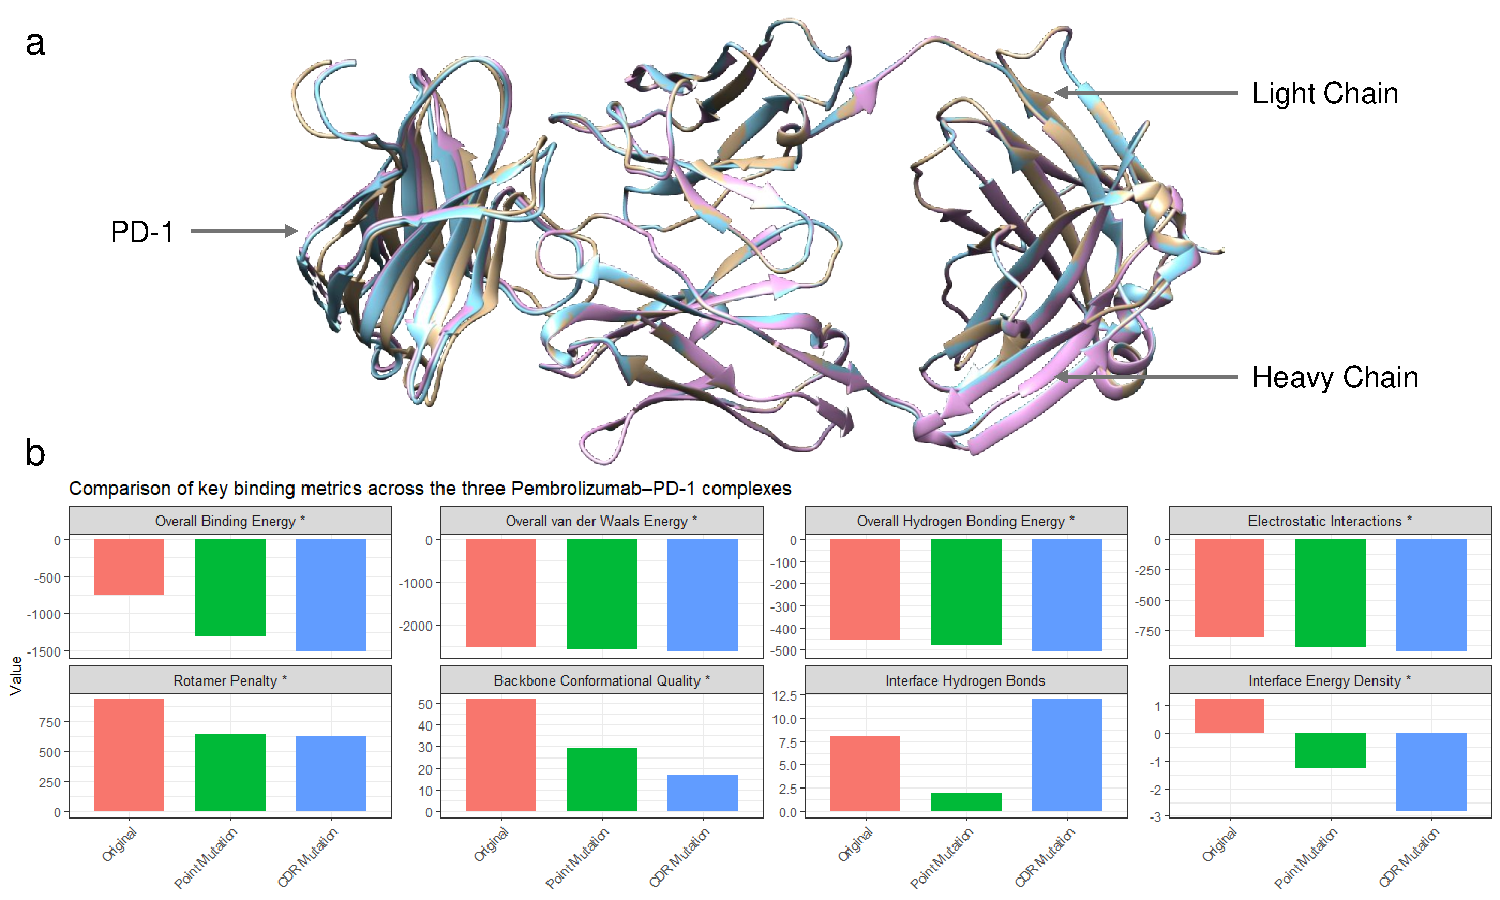
\includegraphics[width=0.8\textwidth]{Figure3.pdf}
\end{center}
\caption{Comparison of the Original Pembrolizumab, Pembrolizumab after Point Mutation and Pembrolizumab after CDR Mutation.}
\textbf{(a)} Aligned structures of the Pembrolizumab–PD-1 complex variants, with the original structure rendered in beige, the point mutation in blue, and the CDR mutation in purple.
\textbf{(b)} Comparison of key binding metrics across the three Pembrolizumab–PD-1 complexes (Original, Point Mutation, and CDR Mutation). Each panel shows one metric, with the asterisk (*) indicating that lower values are more favorable.  
\label{fig:fig3}
\end{figure}

In this analysis, we compared the interaction affinity of the original Pembrolizumab and the mutated Pembrolizumab to PD-1. Figure 3a displays the aligned structures of three Pembrolizumab–PD1 complexes: the original structure (in beige), the point mutation (in blue), and the CDR mutation (in purple). All three models exhibit a high degree of overlap, with similar overall conformations and secondary structures—such as beta sheets, loops, and helices—indicating that the mutations did not disrupt the global fold or backbone architecture.

Despite their overall structural similarity, notable differences emerge at the binding interface with PD1. Both mutated structures (blue and purple) are drawn closer to the receptor compared to the original (beige), suggesting that the mutations enhance the binding affinity. This closer proximity likely results from the introduction of additional favorable interactions—such as extra hydrogen bonds, improved hydrophobic contacts, and stronger electrostatic forces—that stabilize the antibody–receptor complex. These observations are consistent with the scoring and interface analysis results, which indicate improved interaction profiles for the mutated structures. Figure 3b presents histograms comparing key metrics across the three complexes.

The interface analysis comparing the original Pembrolizumab structure with its two modified forms—one harboring a point mutation (affecting two residues) and the other a CDR mutation (affecting four CDRs)—revealed significant improvements in binding energetics upon mutation. The overall binding score of the original complex was –752.43, whereas the point mutation and CDR mutation exhibited substantially lower energies of –1314.11 and –1519.07, respectively, indicating an enhanced binding affinity for the mutated complexes.

Both mutated complexes showed favorable changes in van der Waals and solvation terms. Although the attractive interactions (fa\_atr) remained comparable, the repulsive energies (fa\_rep) were markedly reduced in the mutants, especially in the CDR mutation, which suggests a decrease in steric clashes. Furthermore, the solvation energies decreased slightly for both mutants, contributing to the overall stabilization of the complex. Notably, the electrostatic term (fa\_elec) became increasingly favorable from the original through the point mutant to the CDR mutant, underscoring an improvement in charge complementarity at the interface. Hydrogen bonding metrics further supported these findings. All four hydrogen bond components (short-range backbone, long-range backbone, backbone–sidechain, and sidechain–sidechain) showed progressively more negative values in the mutated complexes. This indicates that both mutations and particularly the CDR mutation, facilitate a more extensive and stronger hydrogen bonding network, which is critical for binding specificity and stability.

In addition to improved interaction energies, the mutated complexes also exhibited better conformational properties. Metrics related to side-chain rotamer quality (fa\_dun) and backbone geometry (p\_aa\_pp, rama\_prepro, and omega) were all more favorable in the mutated forms compared to the original structure. The CDR mutation, in particular, resulted in the lowest penalties, suggesting an optimized interface with reduced conformational strain. Importantly, global structural metrics such as all-atom RMSD and GDT measures remained consistent across all three groups, confirming that the overall architecture of the complexes was preserved despite local interface modifications.

A notable exception was the yhh\_planarity term. While this metric was relatively low in both the original and the point mutant, the CDR mutant exhibited an elevated value. This increase might indicate a deviation in the aromatic side-chain planarity, which could be a compensatory effect of the extensive interface remodeling in the CDR mutation. Although this deviation warrants further structural investigation, it does not appear to compromise the overall binding improvements achieved.

A closer look at the solvent-accessible surface area (SASA) metrics adds further insight into the interface stability. The normalized complex energy becomes progressively more favorable from the original to the point and then to the CDR mutant, with values of –1.337, –2.359, and –2.724, respectively. More striking is the change in the free energy of the separated complex (dG\_separated), which shifts from a positive 57.36 in the original structure to negative values in the mutated forms (–23.14 for the point mutation and –121.61 for the CDR mutation). When normalized by SASA, these improvements suggest that the binding interface becomes energetically more stable per unit area with mutation. Although the point mutation results in a reduced buried interface—indicated by a lower overall dSASA\_int—this comes at the cost of potentially losing some hydrophobic and polar interactions. In contrast, the CDR mutation maintains a larger buried interface that is comparable to the original while still enhancing the balance of hydrophobic and polar contributions. This balance is further reflected in the more favorable per-residue energy values and an increased number of hydrogen bonds at the interface.

The point mutation leads to a considerable enhancement in interface energetics by reducing steric clashes and improving hydrogen bonding and electrostatic interactions. However, the CDR mutation, which involves a broader alteration in the binding regions, delivers a more pronounced optimization across multiple energy components. The deeper energy minimization and improved hydrogen bonding network observed in the CDR mutant indicate that modifications within the CDR can have a substantial positive impact on binding affinity.

Taken together, the analysis indicates that both the point mutation and the CDR mutation contribute to a more optimized and stable interface. The point mutation primarily reduces steric clashes and improves hydrogen bond satisfaction by decreasing the interface area, while the CDR mutation achieves a more comprehensive improvement by not only enhancing the energetics but also preserving a large, balanced binding surface. The overall superior performance of CDR mutation across binding energy, SASA, and hydrogen bonding metrics makes it the more effective strategy for optimizing the complex’s stability.

\section{Discussion}

This study illustrates the significant potential of computer-aided drug discovery (CADD) techniques, particularly those offered by the Rosetta suite, in the design and optimization of therapeutic antibodies targeting the PD-1 receptor. Our structure-based drug design (SBDD) approach enabled us to screen three FDA-approved PD-1 inhibitors—Pembrolizumab, Nivolumab, and Cemiplimab—and identify Pembrolizumab as the most promising candidate based on its favorable binding energy and stable interaction profile with PD-1.

Detailed binding analysis revealed that key residues in Pembrolizumab contribute to both stabilizing and destabilizing interactions. Unfavorable steric clashes and electrostatic repulsion, particularly involving residues such as 53 L (TYR) and 59 H (ASN), emerged as potential targets for optimization. Subsequent mutagenesis studies, involving both point mutations and broader CDR modifications, significantly enhanced the interaction profile of Pembrolizumab. The mutated complexes demonstrated improved binding energy, with enhanced van der Waals and electrostatic interactions, increased hydrogen bonding, and a more compact interface, ultimately leading to a more favorable overall energy state.

The solvent-accessible surface area (SASA) analysis further reinforced these findings. The mutated complexes, especially the one with CDR modifications, showed a more favorable normalized complex energy and a substantially improved free energy of the separated complex, indicating that the binding interface becomes energetically more stable per unit area. Additionally, while the point mutation resulted in a reduced buried interface area, the CDR mutation maintained a larger, well-balanced interface that preserves both hydrophobic and polar interactions, thereby contributing to enhanced stability.

Collectively, these results highlight the utility of computational optimization in refining antibody–receptor interactions at the molecular level. The improved binding affinity and stability of the mutated Pembrolizumab-PD-1 complex position it as a stronger candidate for further preclinical investigation. This research not only validates the effectiveness of Rosetta-based techniques in antibody engineering but also underscores the potential of CADD to accelerate the development of more effective PD-1-targeted cancer therapies.

\section{Conclusion}

In this study, we successfully utilized computer-aided drug discovery (CADD) techniques, particularly the Rosetta suite, to optimize therapeutic antibodies targeting the PD-1 receptor. While the results provide promising insights into improving antibody binding affinity and stability, several limitations should be considered in interpreting these findings.

Firstly, the experimental dissociation constants (K\_d) for Pembrolizumab, Nivolumab, and Cemiplimab were reported as 27 pM, 4.06 nM, and 0.6 nM, respectively \cite{jeong2022}. The corresponding Gibbs free energy ($\Delta G$) values were calculated for each of these antibodies, yielding $\Delta G$ values of approximately 14.41 kcal/mol for Pembrolizumab, 11.44 kcal/mol for Nivolumab, and 12.57 kcal/mol for Cemiplimab. The ranking of the docking scores perfectly matches the rank of the experimental data, with Pembrolizumab having the most favorable binding, followed by Cemiplimab and Nivolumab. However, the absolute values of the docking energies do not align with the experimental $\Delta G$ values, suggesting that while docking simulations can accurately predict the relative binding affinities of molecules, they may not provide precise quantitative predictions. This discrepancy underscores the need for experimental validation to complement docking results and ensure a more accurate assessment of binding affinity.

Secondly, a promising therapeutic antibody must not only exhibit strong binding affinity to its receptor but also possess desirable pharmacokinetic (PK) and pharmacodynamic (PD) properties. These include factors like half-life, tissue distribution, and immune system interactions. In this study, the focus was primarily on improving the binding affinity of the antibody to PD-1, but further optimization should also consider these PK/PD properties. A good affinity does not necessarily equate to therapeutic success if the molecule cannot effectively reach the target site or remain active long enough to exert its effects.

Another limitation is the lack of molecular dynamics (MD) simulations to assess the stability of the antibody-receptor complex over time. While the Rosetta suite excels at docking and structure optimization, it lacks a dedicated module for molecular dynamics simulations, which are critical for understanding the long-term stability, flexibility, and conformational changes of the antibody-receptor complex. Molecular dynamics simulations could provide valuable insights into the dynamic behavior of the drug and its interactions, enhancing the overall prediction of its in vivo performance.

For future research, the use of other CADD pipelines should be considered to complement Rosetta's docking and optimization capabilities. Molecular dynamics simulations with tools like GROMACS \cite{pall2020} or AMBER \cite{salomonferrer2013} would be useful to simulate the time-dependent behavior of the antibody-receptor complex, providing more information on its stability and flexibility. AutoDock Vina \cite{eberhardt2021} is another alternative docking platform that could complement Rosetta by offering different algorithms and scoring functions, potentially yielding more robust predictions. Additionally, advanced machine learning-based tools like DeepChem \cite{Ramsundar2019} could be leveraged for LBDD to predict protein-ligand interactions and protein structures more efficiently, providing a broader context for the optimization process. LigandScout \cite{wolber2006} is another tool that can be used in LBDD, providing a structure-based approach to identifying bioactive ligand fragments and optimizing their interactions with the target receptor. LBDD’s ability to apply QSAR modeling and other ligand-based methods can complement the structural insights from Rosetta by optimizing the ligand's chemical properties and its interaction profile with the target. Combining these methods can provide a more comprehensive understanding of antibody behavior, addressing both the static binding affinity and the dynamic nature of the complex.

Furthermore, experimental validation of the new drug candidates is essential. Testing the optimized antibody in vitro and in vivo will provide the necessary biological data to confirm its efficacy, stability, and pharmacokinetic properties, bridging the gap between computational predictions and real-world applications.

In conclusion, while the study successfully demonstrates the potential of Rosetta-based optimization for PD-1-targeted therapies, the limitations highlighted above suggest that a multi-faceted approach, combining CADD with experimental research, is necessary to fully optimize and validate new therapeutic antibodies.

\begin{thebibliography}{99}

\bibitem{DiMasi2003} DiMasi, J. A., Hansen, R. W., \& Grabowski, H. G. (2003). The price of innovation: new estimates of drug development costs. \textit{Journal of Health Economics, 22}(2), 151--185.

\bibitem{Paul2010} Paul, S. M., Mytelka, D. S., Dunwiddie, C. T., Persinger, C. C., Munos, B. H., Lindborg, S. R., \& Schacht, A. L. (2010). How to improve R\&D productivity: the pharmaceutical industry's grand challenge. \textit{Nature Reviews Drug Discovery, 9}(3), 203--214.

\bibitem{Kitchen2004} Kitchen, D. B., Decornez, H., Furr, J. R., \& Bajorath, J. (2004). Docking and scoring in virtual screening for drug discovery: methods and applications. \textit{Nature Reviews Drug Discovery, 3}(11), 935--949.

\bibitem{Lionta2014} Lionta, E., Spyrou, G., Vassilatis, D. K., \& Cournia, Z. (2014). Structure-based virtual screening for drug discovery: principles, applications and recent advances. \textit{Current Topics in Medicinal Chemistry, 14}(16), 1923--1938.

\bibitem{Sliwoski2014} Sliwoski, G., et al. (2014). Computational methods in drug discovery. \textit{Pharmacological Reviews, 66}(1), 334--395. \url{https://doi.org/10.1124/pr.112.007336}

\bibitem{Kuhn2016} Kuhn, L. A., et al. (2016). Advances in protein--ligand docking and virtual screening. \textit{Journal of Chemical Information and Modeling, 56}(7), 1259--1267. \url{https://doi.org/10.1021/acs.jcim.6b00169}

\bibitem{Moult2019} Moult, J., et al. (2019). Critical assessment of methods of protein structure prediction (CASP) -- round XII. \textit{Proteins: Structure, Function, and Bioinformatics, 87}(12), 1600--1612. \url{https://doi.org/10.1002/prot.25739}

\bibitem{Leaver-Fay2011} Leaver-Fay, A., Tyka, M., Lewis, S. M., Lange, O. F., Thompson, J., Jacak, R., ... \& Kuhlman, B. (2011). Rosetta3: an object‐oriented software suite for the simulation and design of macromolecules. \textit{Methods in Enzymology, 487}, 545--574.

\bibitem{leman2020} Leman, J. K., et al. (2020). Macromolecular modeling and design in Rosetta: recent methods and frameworks. \textit{Nature Methods, 17}(7), 665--680. \url{https://doi.org/10.1038/s41592-020-0848-2}

\bibitem{Alford2017} Alford, R. F., et al. (2017). The Rosetta All-Atom Energy Function for Protein Design and Evaluation. \textit{Journal of Chemical Theory and Computation, 13}(6), 1995--2009. \url{https://doi.org/10.1021/acs.jctc.7b00244}

\bibitem{meiler2006} Meiler, J., \& Baker, D. (2006). ROSETTALIGAND: protein–small molecule docking with full side-chain flexibility. \textit{Proteins: Structure, Function, and Bioinformatics, 65}(3), 538--548. \url{https://doi.org/10.1002/prot.21086}

\bibitem{park2019} Park, H., et al. (2019). Simultaneous optimization of biomolecular energy functions on features from small molecules and macromolecules. \textit{Journal of Chemical Theory and Computation, 15}(9), 5113--5127. \url{https://doi.org/10.1021/acs.jctc.9b00583}

\bibitem{leaver2013} Leaver-Fay, A., et al. (2013). Computational design of ligand-binding proteins with high affinity and selectivity. \textit{Nature Chemical Biology, 9}(7), 506--510. \url{https://doi.org/10.1038/nchembio.1251}

\bibitem{baek2021} Baek, M., et al. (2021). Accurate prediction of protein structures and interactions using a three-track neural network. \textit{Science, 373}(6557), 871--876. \url{https://doi.org/10.1126/science.abj8754}

\bibitem{Dong2002} Dong, H., et al. (2002). Tumor-associated B7-H1 promotes T-cell apoptosis: A potential mechanism of immune evasion. \textit{Nature Medicine, 8}(8), 793--800. \url{https://doi.org/10.1038/nm730}

\bibitem{Topalian2015} Topalian, S. L., et al. (2015). Safety, activity, and immune correlates of anti--PD-1 antibody in cancer. \textit{New England Journal of Medicine, 366}(26), 2443--2454. \url{https://doi.org/10.1056/NEJMoa1200690}

\bibitem{Tan2016} Tan, S., Chen, D., Liu, K., et al. (2016). Crystal clear: Visualizing the intervention mechanism of the PD-1/PD-L1 interaction by two cancer therapeutic monoclonal antibodies. \textit{Protein \& Cell, 7}, 866--877. \url{https://doi.org/10.1007/s13238-016-0337-7}

\bibitem{Chen2019} Chen, D., Tan, S., Zhang, H., et al. (2019). The FG Loop of PD-1 Serves as a “Hotspot” for Therapeutic Monoclonal Antibodies in Tumor Immune Checkpoint Therapy. \textit{iScience, 14}, 113--124. \url{https://doi.org/10.1016/j.isci.2019.03.017}

\bibitem{pettersen2004} Pettersen, E. F., Goddard, T. D., Huang, C. C., Couch, G. S., Greenblatt, D. M., Meng, E. C., \& Ferrin, T. E. (2004). UCSF Chimera--a visualization system for exploratory research and analysis. \textit{Journal of Computational Chemistry, 25}(13), 1605--1612. \url{https://doi.org/10.1002/jcc.20084}

\bibitem{lee2016} Lee, J. Y., Lee, H. T., Shin, W., Chae, J., Choi, J., Kim, S. H., Lim, H., Won Heo, T., Park, K. Y., Lee, Y. J., Ryu, S. E., Son, J. Y., Lee, J. U., \& Heo, Y. S. (2016). Structural basis of checkpoint blockade by monoclonal antibodies in cancer immunotherapy. \textit{Nature Communications, 7}, 13354. \url{https://doi.org/10.1038/ncomms13354}

\bibitem{tan2017} Tan, S., Zhang, H., Chai, Y., Song, H., Tong, Z., Wang, Q., Qi, J., Wong, G., Zhu, X., Liu, W. J., Gao, S., Wang, Z., Shi, Y., Yang, F., Gao, G. F., \& Yan, J. (2017). An unexpected N-terminal loop in PD-1 dominates binding by nivolumab. \textit{Nature Communications, 8}, 14369. \url{https://doi.org/10.1038/ncomms14369}

\bibitem{lu2022} Lu, D., Xu, Z., Zhang, D., Jiang, M., Liu, K., He, J., Ma, D., Ma, X., Tan, S., Gao, G. F., \& Chai, Y. (2022). PD-1 N58-Glycosylation-Dependent Binding of Monoclonal Antibody Cemiplimab for Immune Checkpoint Therapy. \textit{Frontiers in Immunology, 13}, 826045. \url{https://doi.org/10.3389/fimmu.2022.826045}

\bibitem{shapovalov2011} Shapovalov, M. V., \& Dunbrack, R. L., Jr. (2011). A smoothed backbone-dependent rotamer library for proteins derived from adaptive kernel density estimates and regressions. \textit{Structure}, 19(6), 844-858. https://doi.org/10.1016/j.str.2011.03.019

\bibitem{jeong2022} Jeong, T. J., Lee, H. T., Gu, N., Jang, Y. J., Choi, S. B., Park, U. B., Lee, S. H., \& Heo, Y. S. (2022). The High-Resolution Structure Reveals Remarkable Similarity in PD-1 Binding of Cemiplimab and Dostarlimab, the FDA-Approved Antibodies for Cancer Immunotherapy. \textit{Biomedicines}, 10(12), 3154. https://doi.org/10.3390/biomedicines10123154

\bibitem{pall2020} Páll, S., Zhmurov, A., Bauer, P., Abraham, M., Lundborg, M., Gray, A., Hess, B., \& Lindahl, E. (2020). Heterogeneous parallelization and acceleration of molecular dynamics simulations in GROMACS. \textit{J. Chem. Phys.}, 153(13), 134110. https://doi.org/10.1063/5.0018516

\bibitem{salomonferrer2013} Salomon-Ferrer, R., et al. (2013). An Overview of the Amber Biomolecular Simulation Package. \textit{WIREs Computational Molecular Science}, 3(2), 198–210. https://doi.org/10.1002/wcms.1121

\bibitem{eberhardt2021} Eberhardt, J., Santos-Martins, D., Tillack, A. F., \& Forli, S. (2021). AutoDock Vina 1.2.0: New Docking Methods, Expanded Force Field, and Python Bindings. \textit{Journal of Chemical Information and Modeling}.

\bibitem{Ramsundar2019}
Bharath Ramsundar, Peter Eastman, Patrick Walters, Vijay Pande, Karl Leswing, Zhenqin Wu. 
\textit{Deep Learning for the Life Sciences}. O'Reilly Media, 2019. 
\url{https://www.amazon.com/Deep-Learning-Life-Sciences-Microscopy/dp/1492039837}

\bibitem{wolber2006}
Wolber, G., Langer, T. LigandScout: 3-D Pharmacophores Derived from Protein-Bound Ligands and Their Use as Virtual Screening Filters. \textit{Journal of Chemical Information and Modeling}, 45(1), 160–169 (2004). \url{https://doi.org/10.1021/ci034243}.

\end{thebibliography}

\end{document}
